% StorePulse AI -- project presentation (Beamer, 16:9, metropolis theme).
% Build: see README.md (tectonic slides.tex). Speaker notes: uncomment the \setbeameroption line below.
\documentclass[aspectratio=169,11pt]{beamer}
\usetheme[progressbar=frametitle,numbering=fraction,block=fill]{metropolis}
\ifdefined\withnotes
  \usepackage{pgfpages}
  \setbeameroption{show notes on second screen=right}  % slides-notes.tex: slide + speaker notes
\fi

\usepackage{booktabs}
\usepackage{graphicx}
\usepackage{tikz}
\usetikzlibrary{arrows.meta,positioning,shapes.geometric,calc}
\usepackage{xurl}

% Restrained palette: navy text/headers, one blue accent, green for "best", orange for baselines.
\definecolor{navy}{HTML}{1B2A4A}
\definecolor{accent}{HTML}{0072B2}
\definecolor{good}{HTML}{009E73}
\definecolor{base}{HTML}{D55E00}
\definecolor{soft}{HTML}{F2F5FA}
\setbeamercolor{frametitle}{bg=navy,fg=white}
\setbeamercolor{progress bar}{fg=accent,bg=soft}
\setbeamercolor{alerted text}{fg=accent}
\setbeamercolor{example text}{fg=good}
\setbeamercolor{block title}{bg=soft,fg=navy}
\setbeamercolor{block body}{bg=soft!60}
\setbeamerfont{footnote}{size=\tiny}
\setbeamerfont{bibliography item}{size=\tiny}
\setbeamerfont{bibliography entry author}{size=\tiny}
\setbeamerfont{bibliography entry title}{size=\tiny}
\setbeamerfont{bibliography entry location}{size=\tiny}
\setbeamerfont{bibliography entry note}{size=\tiny}
\setbeamertemplate{bibliography item}[text]

\newcommand{\src}[1]{\par\vspace{2pt}{\tiny\color{gray}#1}}

\title{StorePulse AI}
\subtitle{Leakage-free retail demand forecasting and store-level planning}
\author{Bilal Shahid}
\institute{\small Mathematics of Business and Industry $\cdot$ Supervisor: Prof.\ Dr.\ Stefanie Vogl\\
Ostbayerische Technische Hochschule Regensburg (OTH Regensburg)}
\date{\small November 2026}
\titlegraphic{\vspace*{-1mm}\hfill
\includegraphics[height=1.5cm]{figures/oth-regensburg-logo.png}}

\begin{document}

% ---------------------------------------------------------------------------------------------------
\maketitle
\note{Introduce yourself and the project. One sentence: StorePulse turns a store's sales history into
forecasts with ranges and then into a concrete weekly plan.}

% ---------------------------------------------------------------------------------------------------
\begin{frame}{The problem}
\begin{columns}[T]
\column{0.55\textwidth}
\begin{itemize}
  \item Every week a store decides \alert{stock} and \alert{staff} from expected demand
  \item Errors cost money both ways: idle labour vs.\ lost sales
  \item Demand depends on weekdays, promotions, holidays, closures
  \item ML wins forecasting competitions on retail data \cite{makridakis2022m5}, but rarely reaches the person who plans the roster
\end{itemize}
\column{0.42\textwidth}
\begin{block}{Project goal}
From an uploaded sales file to forecasts with P10--P90 ranges, a P\&L, a shift plan and ranked
actions---in a multi-tenant web app.
\end{block}
\end{columns}
\note{Motivation: forecasts are only useful if they become decisions. Competitions (M5) show
gradient boosting dominates, but stays in notebooks. Goal G1--G5 from the project docs: multi-tenant,
no-code pipeline, P\&L and workforce planning, no mock data, GPU training and exports.}
\end{frame}

% ---------------------------------------------------------------------------------------------------
\begin{frame}{Research question}
\begin{block}{RQ (formulated for this report)}
With \alert{no test data used for model selection}, does a global gradient-boosted model forecast
daily store sales \alert{significantly} better than the seasonal-naive benchmark across forecast
origins --- and can its forecasts give \alert{cheaper staffing plans} without more understaffing?
\end{block}
\vspace{4pt}
\begin{columns}[T]
\column{0.32\textwidth}\textbf{H1 Accuracy over time}\\\small 8 rolling 28-day origins; Diebold--Mariano and sign test
\column{0.32\textwidth}\textbf{H2 Model differences}\\\small Ensemble, MLP, GRU vs.\ LightGBM; DM test and store bootstrap
\column{0.32\textwidth}\textbf{H3 Planning}\\\small Integer program vs.\ rule plan, judged against realised footfall
\end{columns}
\note{The project documents state goals but no research question. This RQ is phrased so each part
ends in a test or an optimisation result. Key phrase: no test data used for model selection, which
is why the backtest chooses the number of boosting rounds on the 28 days before each test window.}
\end{frame}

% ---------------------------------------------------------------------------------------------------
\begin{frame}{What StorePulse does}
\centering
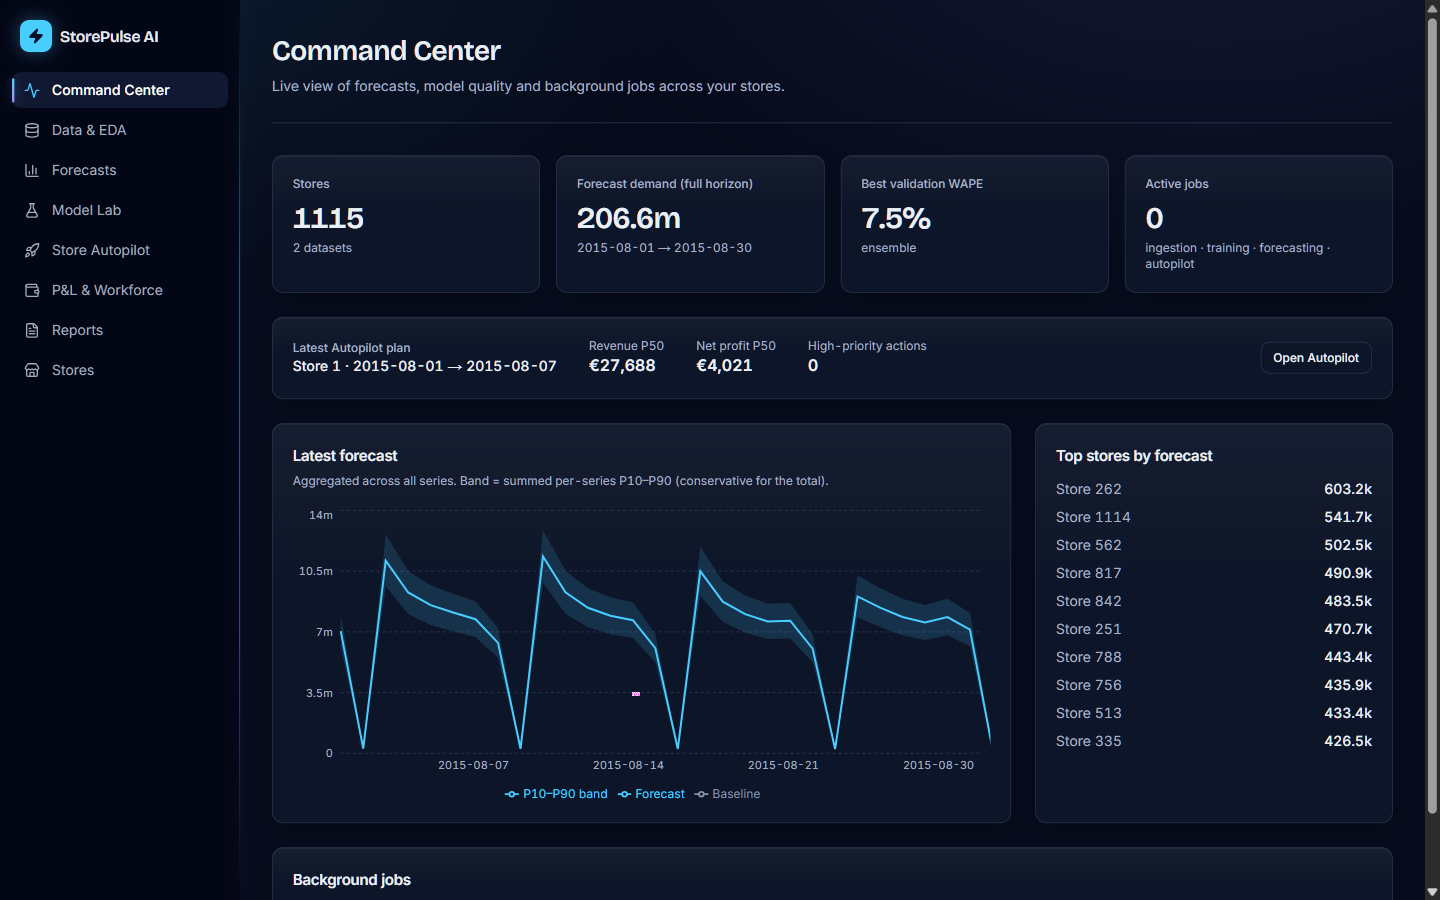
\includegraphics[height=0.74\textheight]{figures/screens/command_center.png}
\src{Command Center, Rossmann demo workspace, all 1,115 stores (screenshot 24 Nov 2026, commit d3fadc8).}
\note{Walk through the eight pages briefly: Data and EDA, Forecasts, Model Lab, Store Autopilot,
P\&L and Workforce, Reports, Stores. Everything here is computed from uploaded data.}
\end{frame}

% ---------------------------------------------------------------------------------------------------
\begin{frame}{Architecture}
\centering
\resizebox{\textwidth}{!}{%
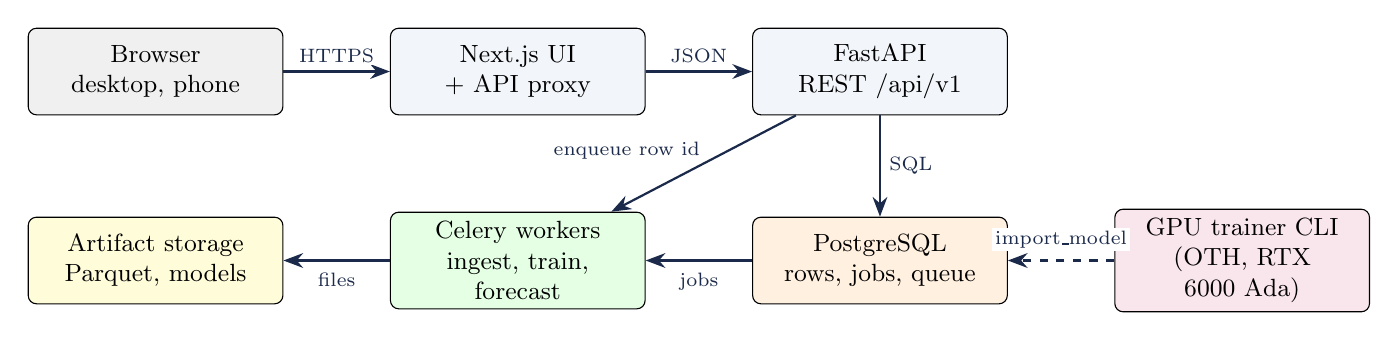
\begin{tikzpicture}[
  box/.style={draw, rounded corners=3pt, align=center, font=\small, text width=30mm, minimum height=11mm},
  arr/.style={-{Stealth[length=2.5mm]}, thick, navy},
  lbl/.style={font=\scriptsize, fill=white, inner sep=1pt}]
\node[box, fill=gray!12]   (browser) at (0,0)      {Browser\\desktop, phone};
\node[box, fill=soft]      (next)    at (4.6,0)    {Next.js UI\\+ API proxy};
\node[box, fill=soft]      (api)     at (9.2,0)    {FastAPI\\REST /api/v1};
\node[box, fill=yellow!15] (store)   at (0,-2.4)   {Artifact storage\\Parquet, models};
\node[box, fill=green!10]  (workers) at (4.6,-2.4) {Celery workers\\ingest, train, forecast};
\node[box, fill=orange!12] (db)      at (9.2,-2.4) {PostgreSQL\\rows, jobs, queue};
\node[box, fill=purple!10] (gpu)     at (13.8,-2.4){GPU trainer CLI\\(OTH, RTX 6000 Ada)};
\draw[arr] (browser) -- node[lbl,above=2pt] {HTTPS} (next);
\draw[arr] (next) -- node[lbl,above=2pt] {JSON} (api);
\draw[arr] (api) -- node[lbl,right=2pt] {SQL} (db);
\draw[arr] (api) -- node[lbl,above left] {enqueue row id} (workers);
\draw[arr] (db) -- node[lbl,below=3pt] {jobs} (workers);
\draw[arr] (workers) -- node[lbl,below=3pt] {files} (store);
\draw[arr, dashed] (gpu) -- node[lbl,above=3pt] {import\_model} (db);
\end{tikzpicture}}
\vspace{6pt}
\begin{itemize}\small
  \item Tasks get only a row id $\Rightarrow$ idempotent, re-runnable; UI polls progress every 2\,s
  \item Every tenant row and storage key carries the organisation id; foreign rows return 404
\end{itemize}
\note{Explain why the API never imports ML code: dispatch by task name keeps the web tier light. The
lean local stack uses PostgreSQL as the queue, so no Redis or Docker is needed on a laptop.}
\end{frame}

% ---------------------------------------------------------------------------------------------------
\begin{frame}{Method: leakage-free direct multi-horizon models}
\begin{columns}[T]
\column{0.5\textwidth}
\begin{itemize}\small
  \item One model predicts every day up to $H$ ahead
  \item Every target feature is lagged by $o=\lceil H/7\rceil\cdot 7$ days (42 for $H{=}42$)
  \item 50 features: calendar, weekday-aligned lags, rolling stats, promo/closure streaks, store type \& assortment aggregates, store metadata
  \item \alert{Scramble test}: change all targets after a cut-off $\Rightarrow$ no earlier feature may change
  \item Closed days: removed from training, forecast exactly 0
\end{itemize}
\column{0.47\textwidth}
\textbf{Model zoo, one interface}\\[2pt]
\footnotesize
\begin{tabular}{@{}ll@{}}
\toprule
Baselines & seasonal naive, ARIMA, SARIMA \\
Trees & LightGBM \cite{ke2017lightgbm} \\
Neural & MLP, GRU \cite{cho2014gru} (PyTorch) \\
Combination & ensemble, weights fitted \\ & on 1st half of validation \\
\bottomrule
\end{tabular}
\end{columns}
\note{Leakage is the most common silent error in forecasting projects; the scramble test makes it
a failing unit test. Tuning with Optuna is scored on an inner split, never on the reported window.}
\end{frame}

% ---------------------------------------------------------------------------------------------------
\begin{frame}{Mathematical formulation}
\begin{columns}[T]
\column{0.5\textwidth}
\textbf{Direct forecast, leakage-free}
\[ \hat y_{i,T+h} = f\bigl(\phi(y_{i,\le T+h-o}),\ \mathbf z_{i,T+h},\ \mathbf s_i\bigr) \]
\small $o=\lceil H/7\rceil\cdot 7 \ \Rightarrow\ T+h-o\le T$ for all $h\le H$; weekday-aligned.
\vspace{6pt}

\normalsize\textbf{Diebold--Mariano}
\[ d_t=\tfrac{\sum_i(|e^A_{it}|-|e^B_{it}|)}{\sum y},\quad
   \mathrm{DM}=\tfrac{\bar d}{\sqrt{\hat\sigma^2_{\mathrm{NW}}/T}} \]
\small HLN small-sample factor, $t_{T-1}$; store bootstrap as cross-check.
\column{0.48\textwidth}
\textbf{Staffing integer program}
\[ \min_{x\in\mathbb Z^J_{\ge0}} \sum_j \ell_j x_j \quad\text{s.t.}\quad \sum_j a_{tj}x_j \ge r_t \]
\small $r_t=\max(m,\lceil F p_t/c\rceil)$ staff needed in hour $t$; templates $j$: start hour,
length 4/6/8\,h (set covering, Dantzig 1954).\\[4pt]
Service level: plan on $\lambda F$, $\lambda=1$ (P50) \ldots\ 1.117 (P90).
\end{columns}
\note{Be ready to derive why the lag offset prevents leakage: o is at least H, so the newest target used
is at the origin. DM aggregates over stores per day because stores share daily shocks. The IP is the
classic shift-scheduling covering model; HiGHS solves each store-day in milliseconds.}
\end{frame}

% ---------------------------------------------------------------------------------------------------
\begin{frame}{Evaluation setup}
\begin{columns}[T]
\column{0.5\textwidth}
\textbf{Data}
\begin{itemize}\small
  \item Rossmann \cite{kaggle2015rossmann}: 1,017,209 store-days, 1,115 stores, 2013--2015
  \item Favorita \cite{kaggle2021storesales}: 3.0\,M rows, 54 stores $\times$ 33 families
\end{itemize}
\textbf{Split}
\begin{itemize}\small
  \item Hold out last $H$ days: 42 d (20 Jun--31 Jul 2015), 30 d (2--31 Jul)
  \item All models of a horizon scored on the same rows
\end{itemize}
\column{0.47\textwidth}
\textbf{Metrics}
\begin{itemize}\small
  \item \alert{WAPE} $=\sum|y-\hat y|/\sum y$ (primary)
  \item RMSSE, RMSPE, RMSE, $R^2$, bias \cite{hyndman2006another}
  \item Hold-out coverage of P10--P90
  \item Latency (ms), job and training time (s)
\end{itemize}
\textbf{Hardware}: RTX 6000 Ada (OTH) for neural nets; laptop i7-8665U for baselines and reruns
\end{columns}
\note{WAPE is defined on zero days (closures) and reads as euros of error per euro sold. In-sample
coverage is inflated by closed days, so only hold-out coverage is reported.}
\end{frame}

% ---------------------------------------------------------------------------------------------------
\begin{frame}{Single split: learned models halve the error}
\begin{columns}[c]
\column{0.52\textwidth}
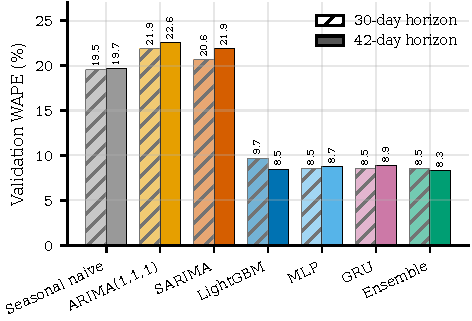
\includegraphics[width=\linewidth]{figures/fig_accuracy.pdf}
\column{0.46\textwidth}
\footnotesize
\begin{tabular}{@{}lrr@{}}
\toprule
WAPE (\%) & 42 d & 30 d \\
\midrule
Seasonal naive & 19.69 & 19.54 \\
ARIMA / SARIMA & 22.6 / 21.9 & 21.9 / 20.6 \\
\midrule
LightGBM & 8.48 & 9.70 \\
MLP & 8.72 & 8.55 \\
GRU & 8.86 & \textbf{8.52} \\
Ensemble & \textbf{8.34} & (= GRU) \\
\bottomrule
\end{tabular}
\end{columns}
\src{All 1,115 stores, identical validation window per horizon. Data: report/data/fig\_accuracy\_source.csv.}
\note{One window per horizon: 51 to 58 percent lower WAPE than the seasonal-naive baseline.
ARIMA/SARIMA are worse than naive in WAPE; they do not use promotions, which lift mean sales by 38.8
percent in this data. Caveat: these runs chose the stopping point on this same window, hence the
backtest on the next slide.}
\end{frame}

% ---------------------------------------------------------------------------------------------------
\begin{frame}{H1: rolling-origin backtest (8 origins, honest stopping)}
\begin{columns}[c]
\column{0.56\textwidth}
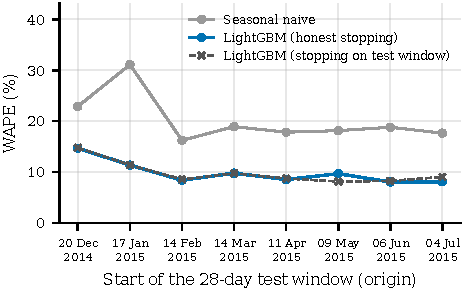
\includegraphics[width=\linewidth]{figures/fig_backtest.pdf}
\column{0.42\textwidth}
\small
\begin{itemize}
  \item LightGBM better at \alert{8 of 8} origins
  \item Mean WAPE \textbf{9.8\,\%} (7.9--11.7) vs.\ \textbf{20.2\,\%} (16.2--24.2)
  \item DM$^\ast=-10.9$, $p<10^{-4}$; sign test $p=0.008$
  \item Stopping on the test window: no systematic gain ($p=0.92$)
  \item Christmas is hardest: 14.7\,\% vs.\ 22.9\,\%
\end{itemize}
\end{columns}
\src{28-day windows, 20 Dec 2014--31 Jul 2015, 242,560 store-days; rounds chosen on the 28 days before each window.}
\note{H1 supported. The single split's 8.5 percent is at the favourable end; 9.8 percent is the
year-round figure. Round counts vary from 66 to 3,050, so early stopping on squared error is a weak
selector, but test-window stopping did not inflate WAPE here.}
\end{frame}

% ---------------------------------------------------------------------------------------------------
\begin{frame}{Uncertainty and combination}
\begin{columns}[T]
\column{0.5\textwidth}
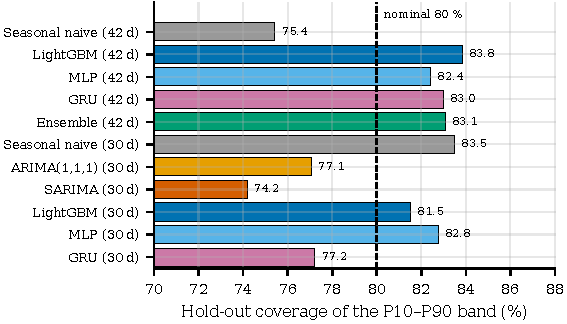
\includegraphics[width=\linewidth]{figures/fig_coverage.pdf}
\small Learned models: 77--84\,\% hold-out coverage (nominal 80\,\%); ARIMA/SARIMA under-cover with bands $>$2$\times$ wider.
\column{0.48\textwidth}
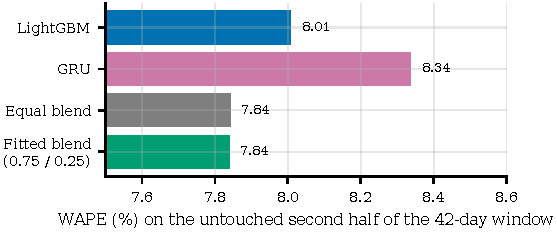
\includegraphics[width=\linewidth]{figures/fig_ensemble.pdf}
\small On the untouched 2nd half of the 42-day window the blend beats both members (7.84 vs.\ 8.01 / 8.34\,\%).
\end{columns}
\note{Bands usable for P10 downside and P90 capacity checks; caveat: the 30-day GRU band is narrow
(77.2 percent). Ensemble weights were fitted on the first half only. The next slide shows that this
small gain is not significant over days.}
\end{frame}

% ---------------------------------------------------------------------------------------------------
\begin{frame}{H2: are the differences real? Diebold--Mariano tests}
\centering\small
\begin{tabular}{@{}llrrr@{}}
\toprule
$H$ & A vs.\ B & $\Delta$WAPE (pp) & DM$^\ast$ & $p$ \\
\midrule
42 & Ensemble vs.\ LightGBM & $-0.14$ & $-1.91$ & 0.063 \\
42 & GRU vs.\ LightGBM & $+0.38$ & $1.69$ & 0.098 \\
30 & GRU vs.\ LightGBM & $-1.18$ & $-4.98$ & \textbf{$<$0.001} \\
30 & GRU vs.\ MLP & $-0.03$ & $-0.10$ & 0.920 \\
30 & LightGBM vs.\ SARIMA & $-10.92$ & $-4.10$ & \textbf{$<$0.001} \\
\bottomrule
\end{tabular}
\vspace{6pt}
\begin{itemize}\small
  \item The ensemble's 0.14-point gain is \alert{not significant over days} ($p=0.063$)
  \item Store bootstrap says ``significant'' --- but it ignores shocks shared by all stores on a day
  \item Neural nets beat LightGBM at 30 days; GRU and MLP are indistinguishable
\end{itemize}
\note{Explain the two tests: bootstrap asks whether the result holds for other stores, DM whether it
holds on other days. With 42 days there are only about 42 independent pieces of evidence.}
\end{frame}

% ---------------------------------------------------------------------------------------------------
\begin{frame}{From forecast to plan: Store Autopilot}
\begin{columns}[c]
\column{0.62\textwidth}
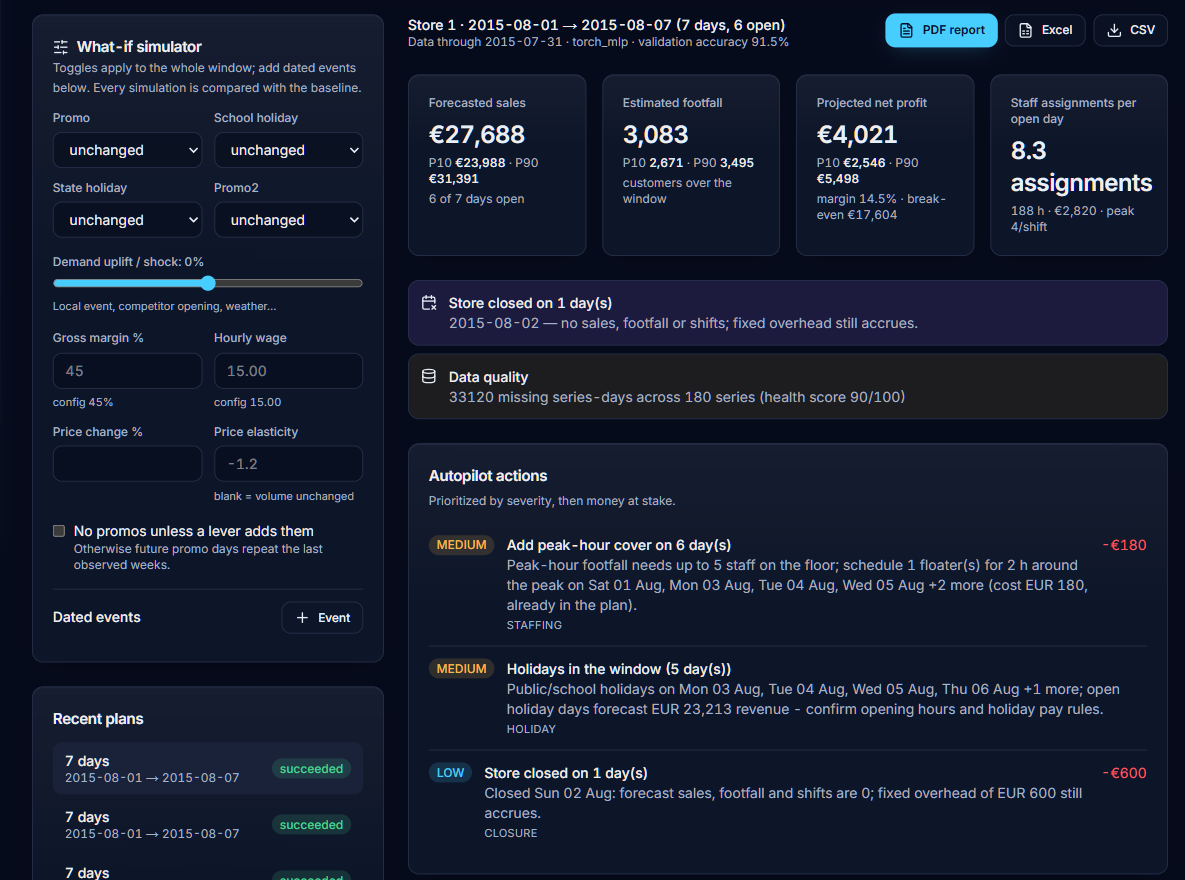
\includegraphics[width=\linewidth]{figures/screens/autopilot_plan.png}
\column{0.36\textwidth}
\small
\begin{itemize}
  \item Revenue, footfall, net profit as P10 / P50 / P90
  \item Break-even $=\frac{\text{labour}+\text{overhead}}{\text{contribution ratio}}$
  \item Shifts: headcount per shift, peak floaters
  \item Ranked actions; what-if levers re-forecast through the model
  \item Every assumption echoed in the output
\end{itemize}
\end{columns}
\src{Store 1, 7-day plan, MLP model. Costs and wages are demo planning values, not real store data.}
\note{Explain that the planning layer is rule-based by design: a manager must understand why the
plan suggests a floater on Saturday. An optimiser is future work.}
\end{frame}

% ---------------------------------------------------------------------------------------------------
\begin{frame}{H3: staffing optimiser vs.\ rules}
\begin{columns}[c]
\column{0.55\textwidth}
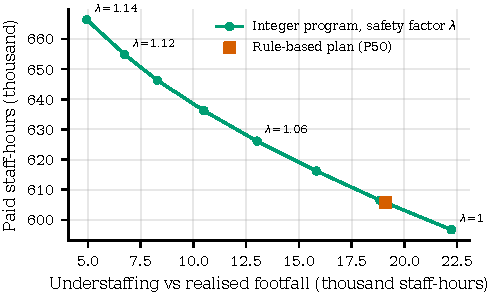
\includegraphics[width=\linewidth]{figures/fig_staffing.pdf}
\column{0.43\textwidth}
\small
\begin{itemize}
  \item 13,420 store-days, judged against \alert{actual} customers
  \item IP on P50: $-1.5\,\%$ hours but $+16\,\%$ understaffing
  \item IP on P90: $+8.1\,\%$ hours, $-65\,\%$ understaffing
  \item At equal understaffing: \alert{same cost} as rules ($+0.00\,\%$)
  \item H3 not supported --- value is choosing the service level
\end{itemize}
\end{columns}
\src{Hourly profile and staffing parameters are planning assumptions (daily data only).}
\note{An honest negative result: the rules' rounding acts as a safety buffer and lies on the
optimiser's frontier. The optimiser makes the cost of service explicit, e.g. lambda 1.06 costs 3.4
percent more hours and removes 32 percent of understaffing.}
\end{frame}

% ---------------------------------------------------------------------------------------------------
\begin{frame}{Interactive and reproducible}
\begin{columns}[T]
\column{0.52\textwidth}
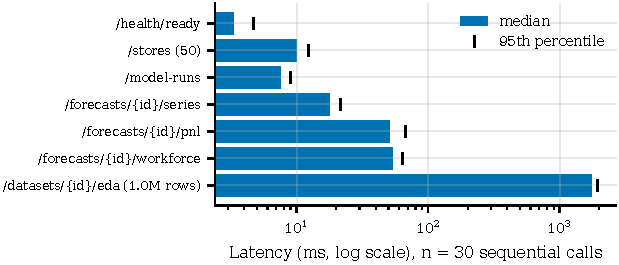
\includegraphics[width=\linewidth]{figures/fig_latency.pdf}
\column{0.46\textwidth}
\small
\begin{itemize}
  \item Forecast, P\&L, workforce: \alert{$\le$70\,ms} (P95); full EDA on 1\,M rows: 1.7\,s
  \item Forecast job (1,115 stores): 9.3\,s median; Autopilot plan: 4.8\,s
  \item LightGBM rerun on the laptop reproduced the GPU host's WAPE \alert{to 4 decimals}
  \item GPU trains the MLP $\approx$57$\times$ faster (10.8\,s vs.\ 614\,s)
  \item 57 automated tests pass (38.5\,s)
\end{itemize}
\end{columns}
\src{Laptop: Intel Core i7-8665U, 24 GB RAM, loopback, 30 sequential calls per endpoint.}
\note{Engineering question: yes on a single client. Concurrency and network latency were not tested.}
\end{frame}

% ---------------------------------------------------------------------------------------------------
\begin{frame}{Limitations and threats to validity}
\begin{itemize}
  \item \textbf{Model selection}: single-split results stopped training on the test window; only LightGBM was re-run honestly
  \item \textbf{Backtest scope}: 8 consecutive origins share training data; neural nets not backtested (CPU cost)
  \item \textbf{Staffing model}: hourly profile assumed (daily data); demo wages and service rates
  \item \textbf{Data sets}: Rossmann store-level; Favorita one model (13.07\,\%); M5 item level not evaluated
  \item \textbf{Robustness}: run-through found all-zero neural forecasts on 1-year history (fixed + test)
\end{itemize}
\note{Be explicit: these limit how far the conclusion generalises. The all-zero bug is a good example
of why an end-to-end run-through belongs in the evaluation.}
\end{frame}

% ---------------------------------------------------------------------------------------------------
\begin{frame}{Future work}
\begin{columns}[T]
\column{0.5\textwidth}
\begin{enumerate}
  \item Honest backtest of neural nets and ensemble on the GPU; honest stopping as default
  \item M5 item-level evaluation, intermittent-demand metrics
  \item Calibrated bands per lead-time week (conformal / quantile heads)
\end{enumerate}
\column{0.5\textwidth}
\begin{enumerate}\setcounter{enumi}{3}
  \item DeepAR / TFT \cite{salinas2020deepar,lim2021tft} under the same protocol
  \item Multi-day roster IP (contracts, breaks, weekly hours) \cite{ernst2004staff} and hourly footfall data
  \item Load tests and a hosted pilot deployment
\end{enumerate}
\end{columns}
\note{Each item maps to one limitation on the previous slide.}
\end{frame}

% ---------------------------------------------------------------------------------------------------
\begin{frame}{Conclusion}
\begin{itemize}
  \item \textbf{H1 supported}: LightGBM halves the benchmark's WAPE at all 8 origins (9.8 vs.\ 20.2\,\%, $p<10^{-4}$)
  \item \textbf{H2 partly}: neural nets beat LightGBM at 30 d ($p<0.001$); the ensemble's gain at 42 d is not significant
  \item \textbf{H3 not supported}: the integer program is not cheaper at equal understaffing --- it prices the service level
  \item Leakage-free direct pipeline with a formal argument and an automated test; bands cover 77--84\,\%
  \item Open: neural backtests on GPU, other data sets, real hourly demand
\end{itemize}
\vfill
\centering\large Thank you --- questions?
\note{Answer to the RQ: yes for forecasting accuracy, large and stable across origins; no for cost
savings from optimised staffing in this setting, where the optimiser's value is explicit pricing of
the service level.}
\end{frame}

% ===================================================================================================
\appendix
\begin{frame}{Backup: full accuracy table (42-day horizon)}
\small\centering
\begin{tabular}{@{}lrrrrrr@{}}
\toprule
Model & WAPE (\%) & RMSE (EUR) & RMSPE & RMSSE & $R^2$ & Fit (s) \\
\midrule
Seasonal naive & 19.69 & 1,682.6 & 0.248 & 0.366 & 0.796 & 0.0 \\
ARIMA(1,1,1) & 22.56 & -- & -- & 0.451 & -- & 727.0 \\
SARIMA & 21.86 & -- & -- & 0.416 & -- & 1,694.5 \\
LightGBM & 8.48 & 803.3 & 0.124 & 0.164 & 0.954 & 11.2 \\
MLP & 8.72 & 831.4 & 0.124 & 0.170 & 0.950 & 10.8 \\
GRU & 8.86 & 845.1 & 0.126 & 0.172 & 0.949 & 43.3 \\
Ensemble & \textbf{8.34} & \textbf{793.3} & 0.122 & \textbf{0.162} & \textbf{0.955} & 43.9 \\
\bottomrule
\end{tabular}
\src{GPU host runs (outputs/rossmann\_h42\_gpu); baselines on the laptop with the same data and window; ``--'' not recorded.}
\end{frame}

\begin{frame}{Backup: error by lead time and weekday}
\begin{columns}[T]
\column{0.5\textwidth}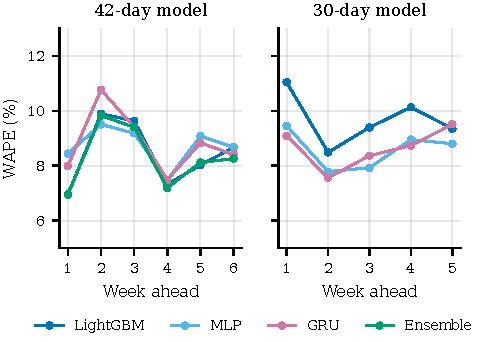
\includegraphics[width=\linewidth]{figures/fig_week_ahead.pdf}
\column{0.5\textwidth}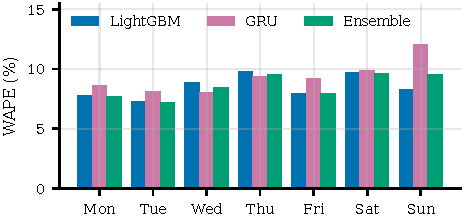
\includegraphics[width=\linewidth]{figures/fig_weekday.pdf}
\end{columns}
\small Error is not monotone in lead time (all features use the full lag offset); neural nets are weakest on rare Sunday openings.
\end{frame}

\begin{frame}{Backup: training time and Favorita product ranking}
\begin{columns}[c]
\column{0.5\textwidth}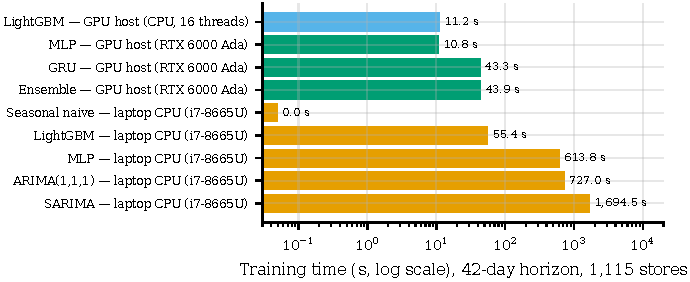
\includegraphics[width=\linewidth]{figures/fig_fit_time.pdf}
\column{0.48\textwidth}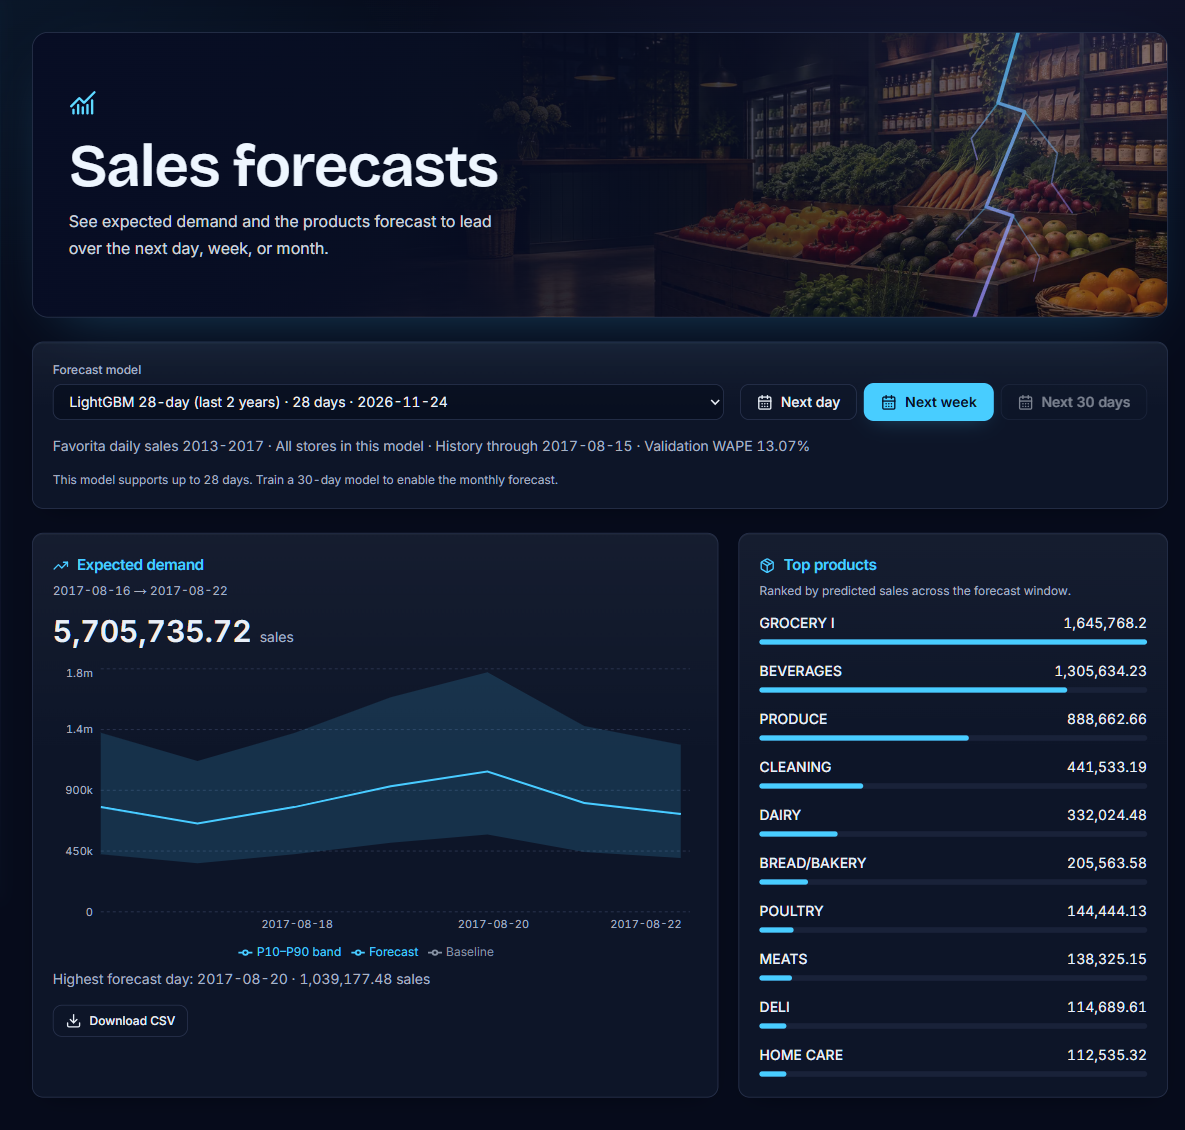
\includegraphics[width=\linewidth]{figures/screens/favorita_forecast.png}
\end{columns}
\end{frame}

\begin{frame}{Backup: Model Lab and exploratory analysis}
\begin{columns}[c]
\column{0.5\textwidth}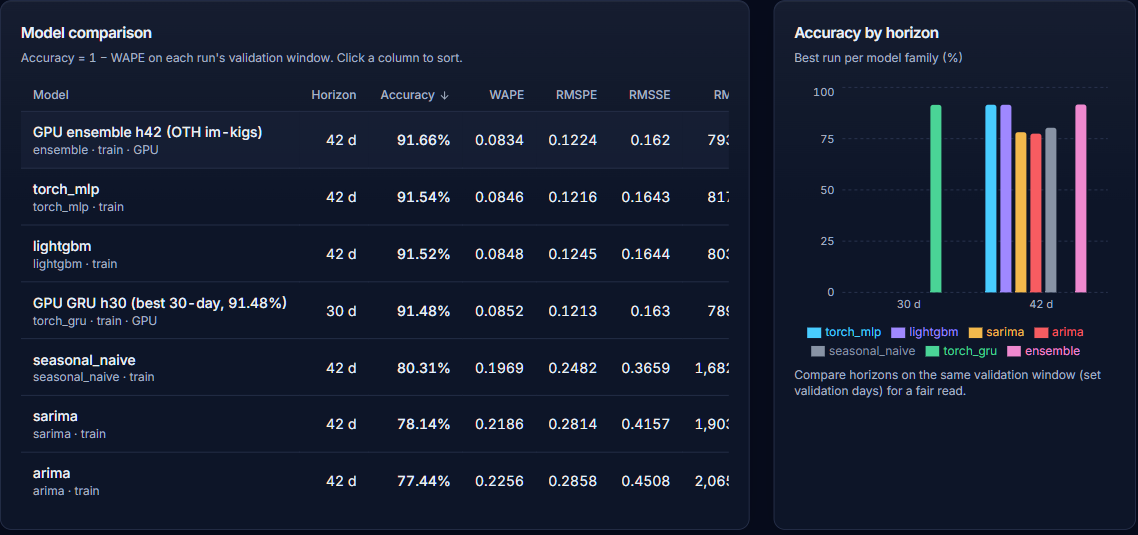
\includegraphics[width=\linewidth]{figures/screens/model_lab_compare.png}
\column{0.5\textwidth}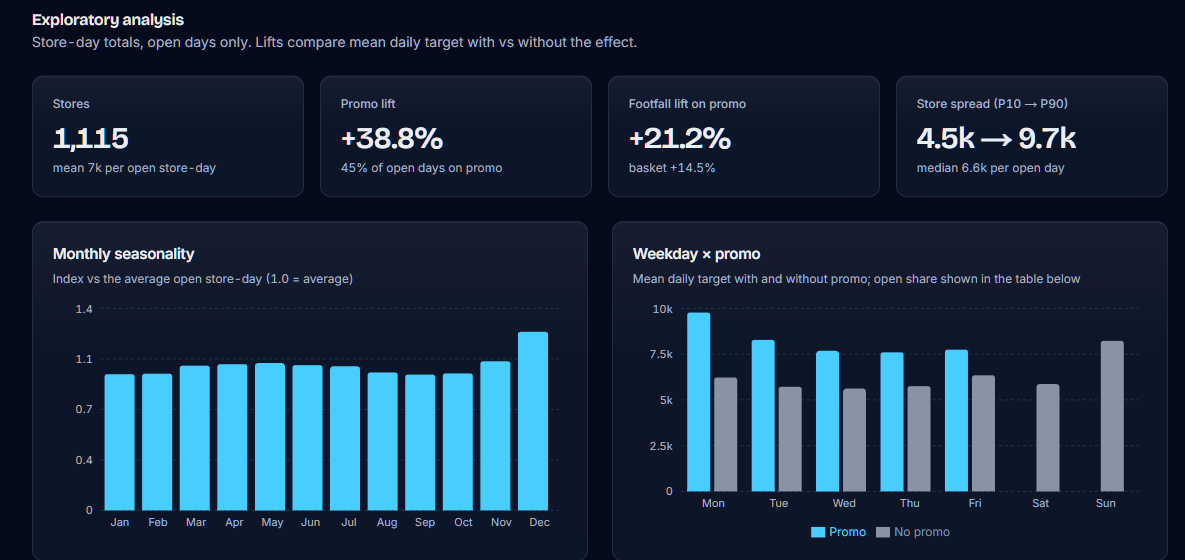
\includegraphics[width=\linewidth]{figures/screens/eda_explore.png}
\end{columns}
\src{Promotions lift mean daily sales by 38.8\,\% and footfall by 21.2\,\% (Rossmann, open days).}
\end{frame}

\begin{frame}{Backup: workflow from upload to plan}
\centering
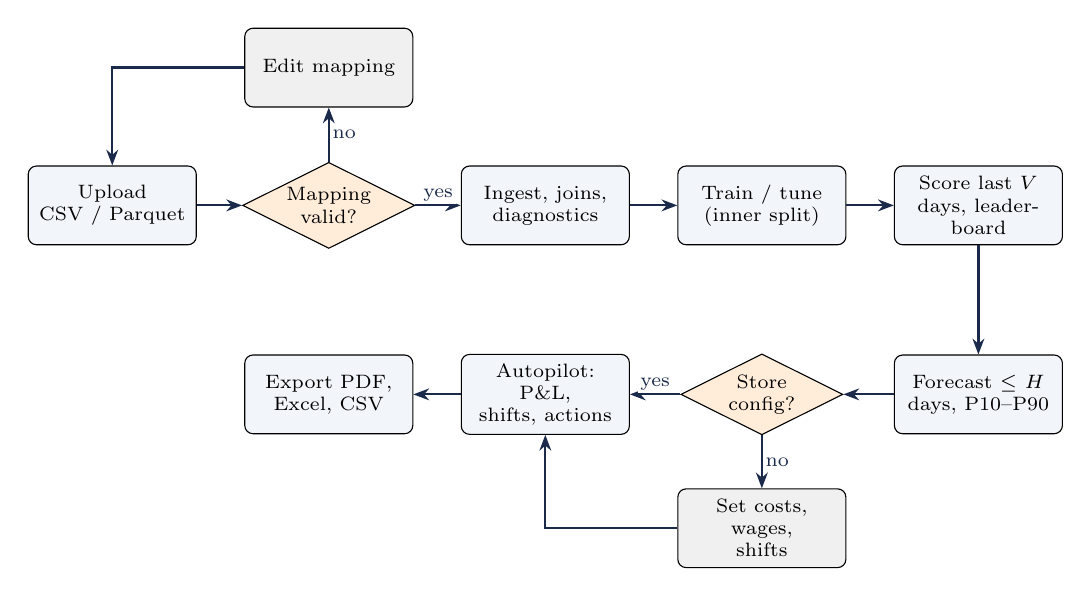
\begin{tikzpicture}[
  st/.style={draw, rounded corners=3pt, fill=soft, align=center, font=\scriptsize, text width=19mm, minimum height=10mm},
  dec/.style={draw, diamond, aspect=2, fill=orange!15, align=center, font=\scriptsize, inner sep=1pt},
  arr/.style={-{Stealth[length=2mm]}, thick, navy},
  lab/.style={font=\scriptsize, fill=white, inner sep=1pt}]
\node[st] (a) at (0,0) {Upload\\CSV / Parquet};
\node[dec] (b) at (2.75,0) {Mapping\\valid?};
\node[st] (c) at (5.5,0) {Ingest, joins,\\diagnostics};
\node[st] (d) at (8.25,0) {Train / tune\\(inner split)};
\node[st] (e) at (11,0) {Score last $V$\\days, leaderboard};
\node[st] (f) at (11,-2.4) {Forecast $\le H$\\days, P10--P90};
\node[dec] (g) at (8.25,-2.4) {Store\\config?};
\node[st] (h) at (5.5,-2.4) {Autopilot: P\&L,\\shifts, actions};
\node[st] (i) at (2.75,-2.4) {Export PDF,\\Excel, CSV};
\node[st, fill=gray!12] (fix) at (2.75,1.75) {Edit mapping};
\node[st, fill=gray!12] (cfg) at (8.25,-4.1) {Set costs, wages,\\shifts};
\draw[arr] (a) -- (b); \draw[arr] (b) -- node[lab,above]{yes} (c); \draw[arr] (c) -- (d); \draw[arr] (d) -- (e);
\draw[arr] (e) -- (f); \draw[arr] (f) -- (g); \draw[arr] (g) -- node[lab,above]{yes} (h); \draw[arr] (h) -- (i);
\draw[arr] (b) -- node[lab,right]{no} (fix); \draw[arr] (fix.west) -| (a.north);
\draw[arr] (g) -- node[lab,right]{no} (cfg); \draw[arr] (cfg.west) -| (h.south);
\end{tikzpicture}
\note{Two decision points users meet: an invalid mapping (the backend explains what to fix) and a
missing store configuration (P\&L needs costs and wages; no values are guessed).}
\end{frame}

\begin{frame}[allowframebreaks]{References}
\tiny
\nocite{makridakis2022m5,ke2017lightgbm,cho2014gru,kaggle2015rossmann,kaggle2021storesales,hyndman2006another,salinas2020deepar,lim2021tft,ernst2004staff}
\bibliographystyle{IEEEtran}
\bibliography{references}
\end{frame}

\end{document}
